En esta sección se analiza el método de síntesis basado en el modelado físico, propuesto por Karplus-Strong.

\subsection{Karplus-Strong básico}
El modelo básico de Karplus-Strong consiste filtrar una forma de onda a través de una linea de retardo. Gracias a esto se logra simular el sonido de una cuerda de guitarra.
\begin{figure}[H]
	\centering
	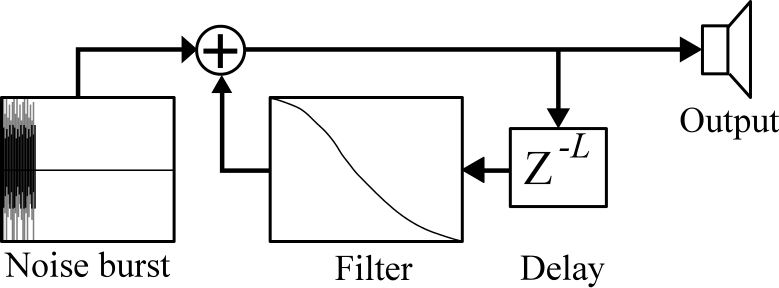
\includegraphics[width=0.8\textwidth]{ImagenesEjercicio4/ksinit.PNG}
\caption{Modelo clásico Karplus-Strong.}
	\label{fig:kscl}
\end{figure}

\subsubsection{Análisis teórico}
Este algoritmo se puede describir por su diagrama en bloques como se ve a continuación.
\begin{figure}[H]
	\centering
	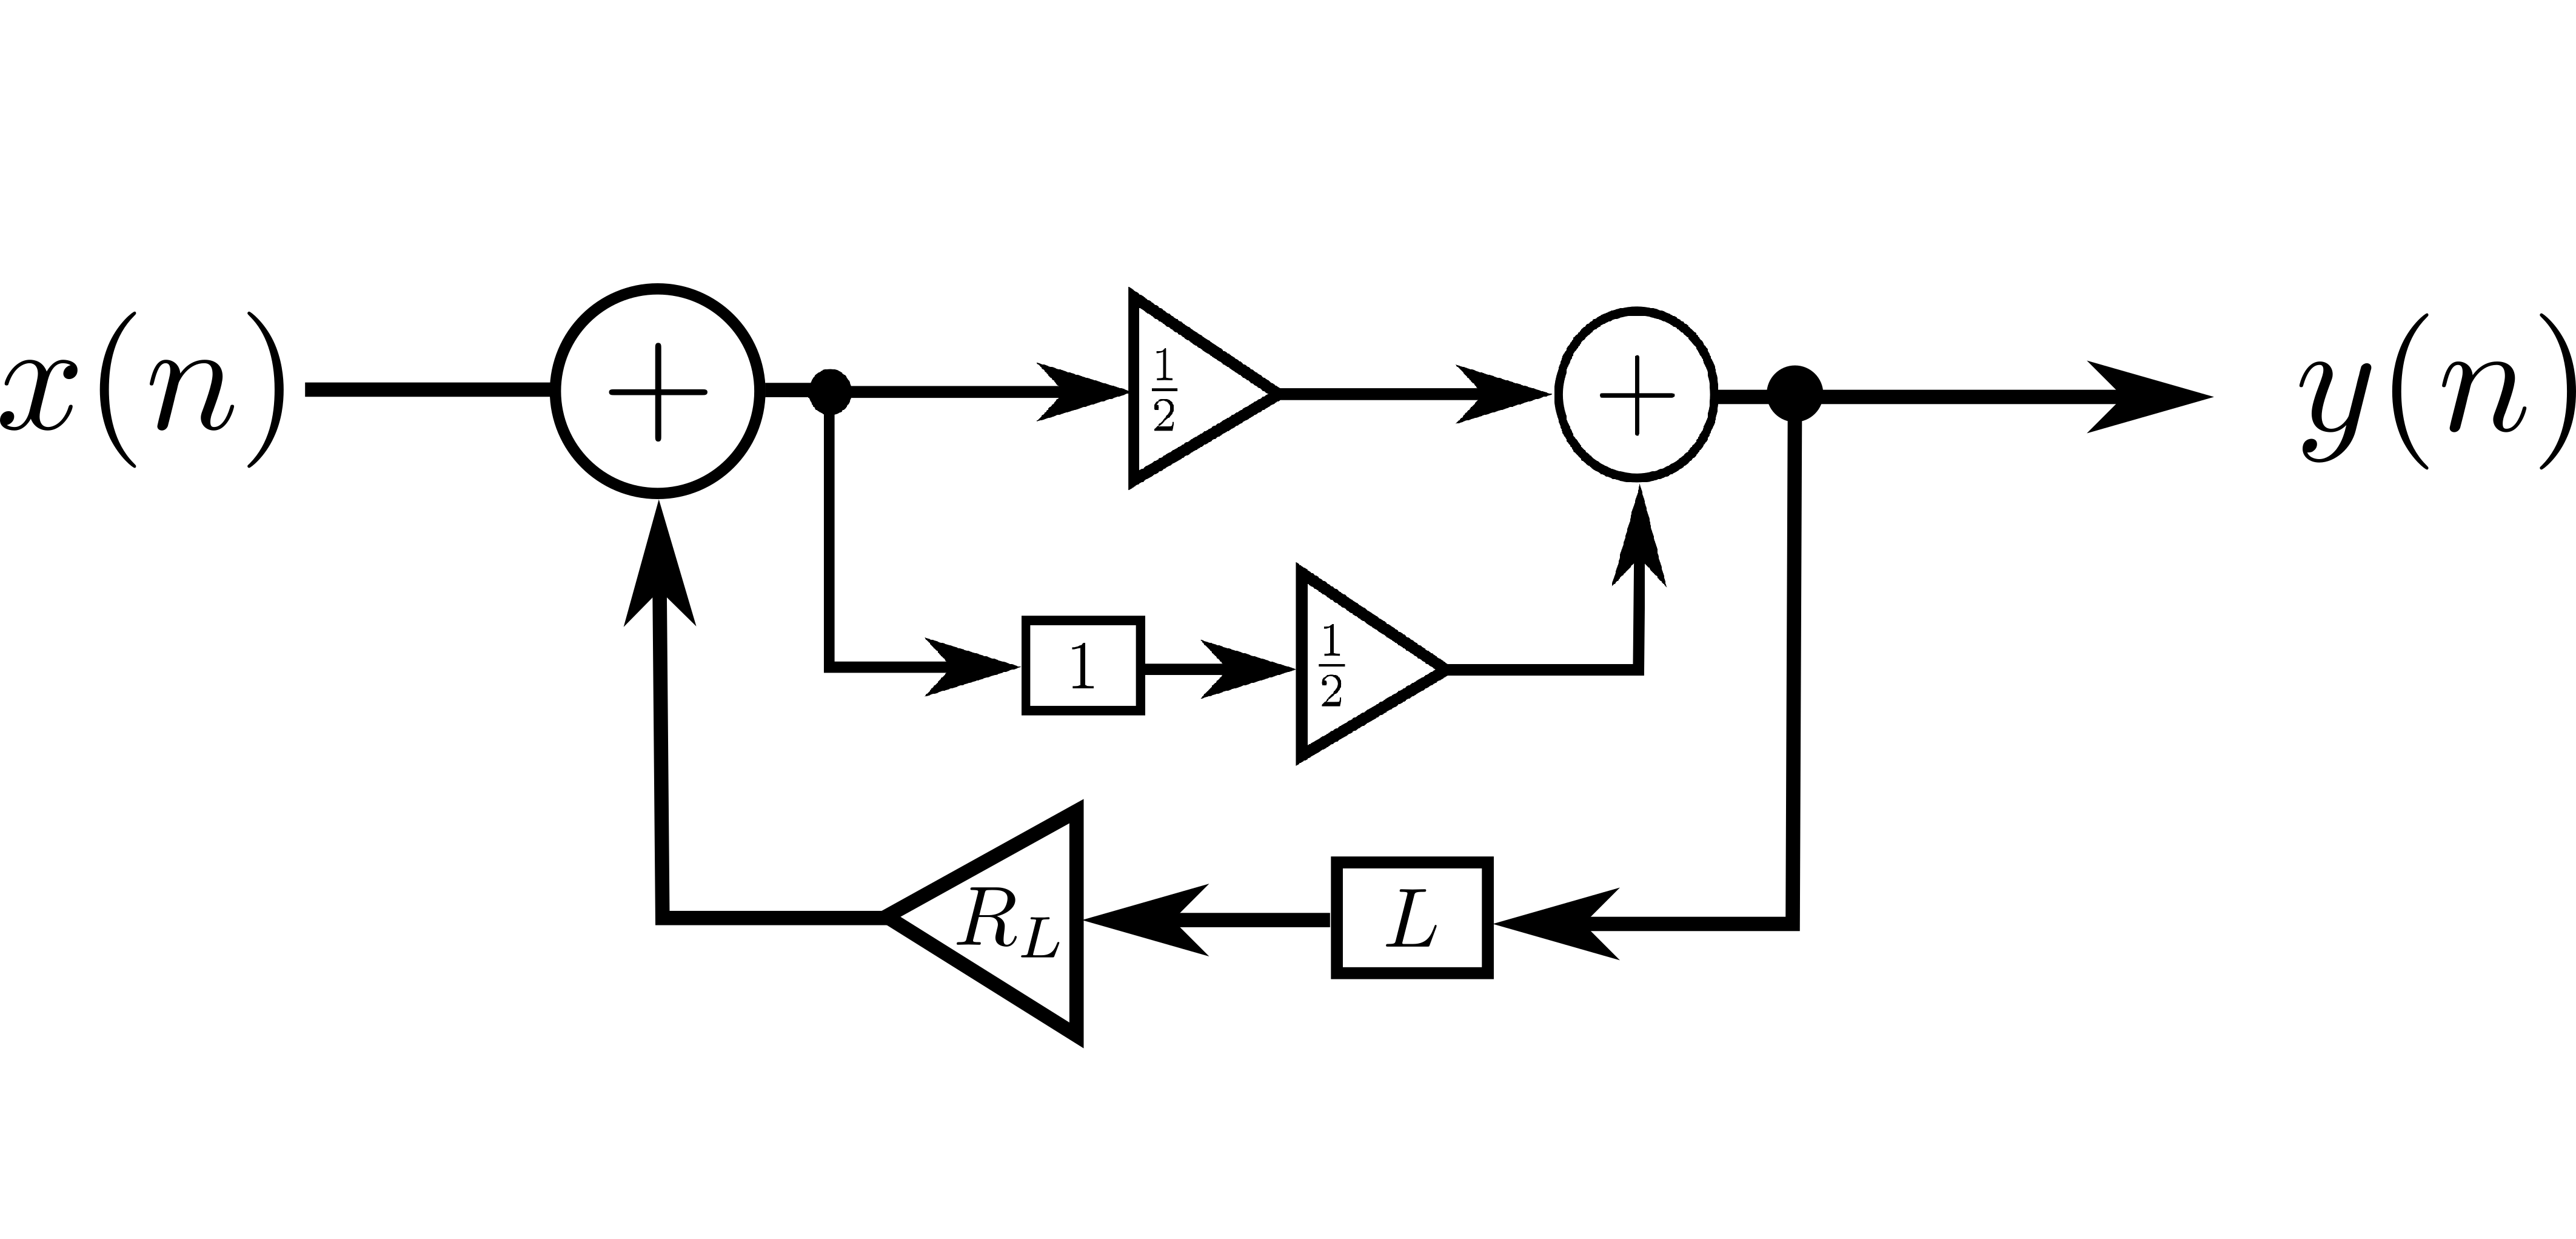
\includegraphics[width=0.8\textwidth]{ImagenesEjercicio4/ksclasic.PNG}
\caption{Algoritmo Karplus-Strong.}
	\label{fig:ksclasico}
\end{figure}
De este diagrama en bloques se puede obtener la ecuación en diferencias:
\begin{align}
y(n) = \frac{1}{2}\cdot x(n) +\frac{1}{2}\cdot x(n-1) + \frac{1}{2}\cdot R_L \cdot y(n-L) + \frac{1}{2}\cdot R_L \cdot y(n-L-1) 
\label{eq:eqdif}
\end{align}

A partir de esta expresión, se calcula su transformada Z y despeja para obtener la transferencia:
\begin{align}
H(z) = \frac{\frac{1}{2} \cdot z^{L+1} +\frac{1}{2} \cdot z^{L} }{z^{L+1} - \frac{R_L}{2} \cdot z - \frac{R_L}{2}}
\label{eq:hzks}
\end{align}  

Vale la pena mencionar que de la Ecuación (\ref{eq:eqdif}) es una ecuación en diferencias que cuenta como condiciones iniciales la ``wavetable'' suministrada por el ruido.

\subsubsection{Análisis singularidades}
Se observa que la Ecuación (\ref{eq:hzks}) cuenta con $L+1$ polos y $L+1$ ceros (de los cuales $L$ de esos se encuentran en el origen). A continuación se muestra un diagrama de polos y ceros del sistema:
\begin{figure}[H]
	\centering
	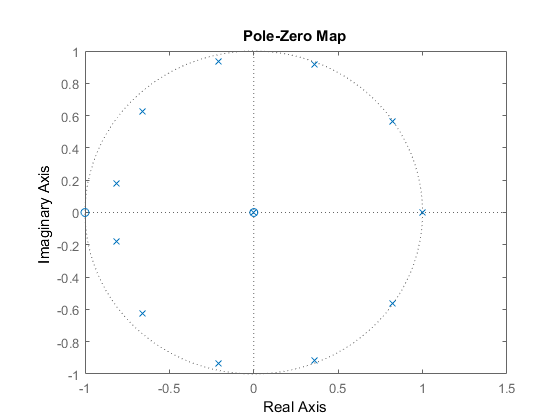
\includegraphics[width=0.8\textwidth]{ImagenesEjercicio4/pzks.PNG}
\caption{Diagrama de polos y ceros.}
	\label{fig:zpdig}
\end{figure}

Adicionalmente, se graficó el diagrama de Bode del sistema.
\begin{figure}[H]
	\centering
	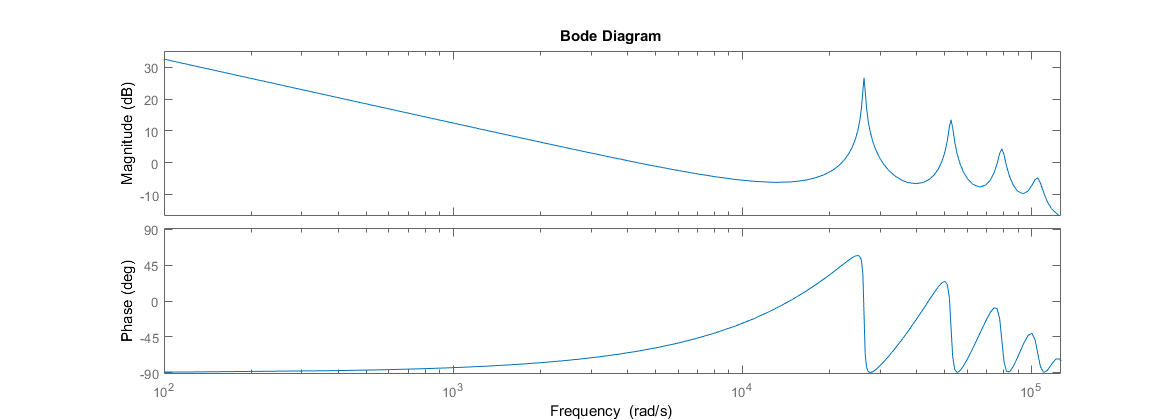
\includegraphics[width=\textwidth]{ImagenesEjercicio4/bodeks.PNG}
	\caption{Diagrama de Bode.}
	\label{fig:bode}
\end{figure}

Considerando que los parámetros eran: $f_s = 44.1 \ kHz$, $L=10$ y $R_L=1$

\subsubsection{Sintonización de frecuencia}
En cuanto a la elección de una frecuencia de oscilación se puede observar en los últimos gráficos que existe un valor de frecuencia, la cual tiene mayor probabilidad de cumplir el criterio de Barkhausen, la cual corresponde a $f_r = \frac{f_s}{L+0.5}$. Esto se debe a que el sistema es la superposición de una linea de retraso $L$ junto con otro sistema de retraso $L+1$. La señal al recorrer el lazo lo hace cada $\frac{L+L+1}{2}$ cambiando esto por frecuencia se obtiene:
\begin{align}
	f_r=\frac{f_s}{L+0.5}
	\label{eq:fr}
\end{align}

\subsubsection{Tipos de ruido}
Se propuso excitar el sistema con distintos tipos de ruido de entrada, siendo estos:
\begin{itemize}
\item Ruido Gaussiano
\item Ruido Uniforme
\item Ruido Binario
\end{itemize}

Primero se aplicó ruido gaussiano de longitud $L=50$, y se obtuvo la siguiente salida:
\begin{figure}[H]
	\centering
	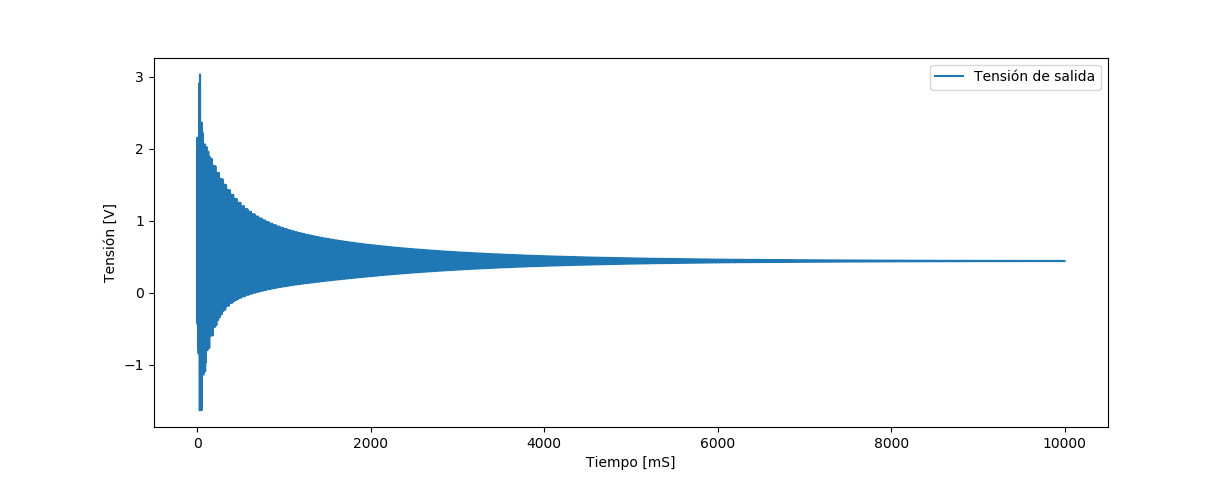
\includegraphics[width=\textwidth]{ImagenesEjercicio4/gaussianResponse.PNG}
\caption{Respuesta a ruido gaussiano, $L=50$.}
	\label{fig:gaussiano}
\end{figure}

Se puede apreciar que la respuesta a este tipo de ruido, parece tener cierta simetría respecto al eje. Algo notable de mencionar es como el sistema se estabiliza para un valor levemente superior a 0. Adicionalmente se realizó un detalle en la imagen:
\begin{figure}[H]
	\centering
	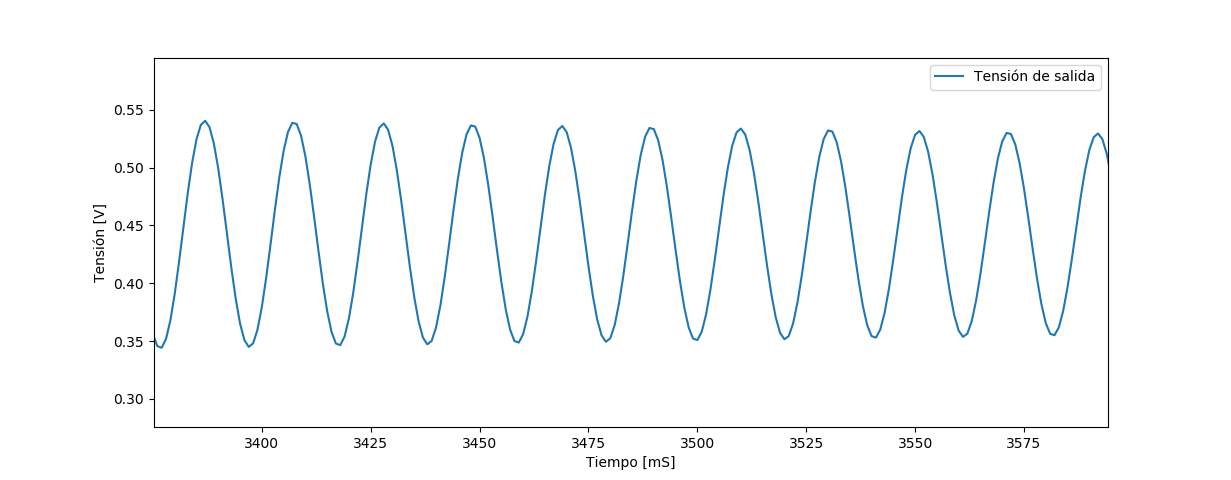
\includegraphics[width=\textwidth]{ImagenesEjercicio4/gaussianResponseDETAIL.PNG}
	\caption{Respuesta a ruido gaussiano detalle, $L=50$.}
	\label{fig:gaussianod}
\end{figure}

En esta, se puede apreciar que el sistema efectivamente se encuentra oscilando, mientras siendo atenuado por una envolvente.

Luego se excitó el sistema con ruido uniforme, obteniendo la siguiente respuesta:
\begin{figure}[H]
	\centering
	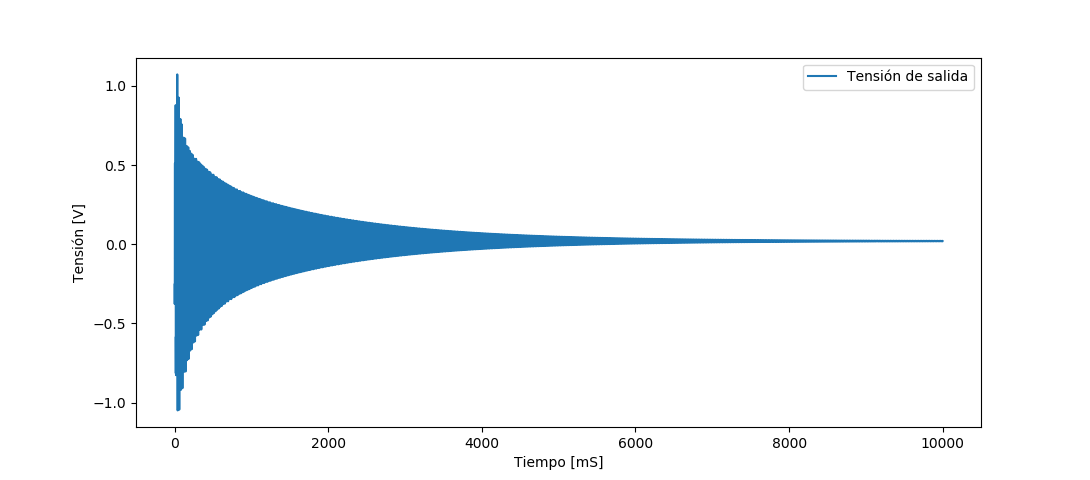
\includegraphics[width=\textwidth]{ImagenesEjercicio4/uniformResponse.PNG}
\caption{Respuesta a ruido uniforme, $L=50$.}
	\label{fig:uniforme}
\end{figure}

Se puede apreciar que la respuesta al ruido uniforme, cuenta con una simetría respecto al eje mas notable que el gaussiano, y un tiempo de decay más lento. Adicionalmente el valor al que tiende es mucho mas cercano a cero.

Luego, de la misma forma que para el gaussiano, se realizó un detalle en la figura:
\begin{figure}[H]
	\centering
	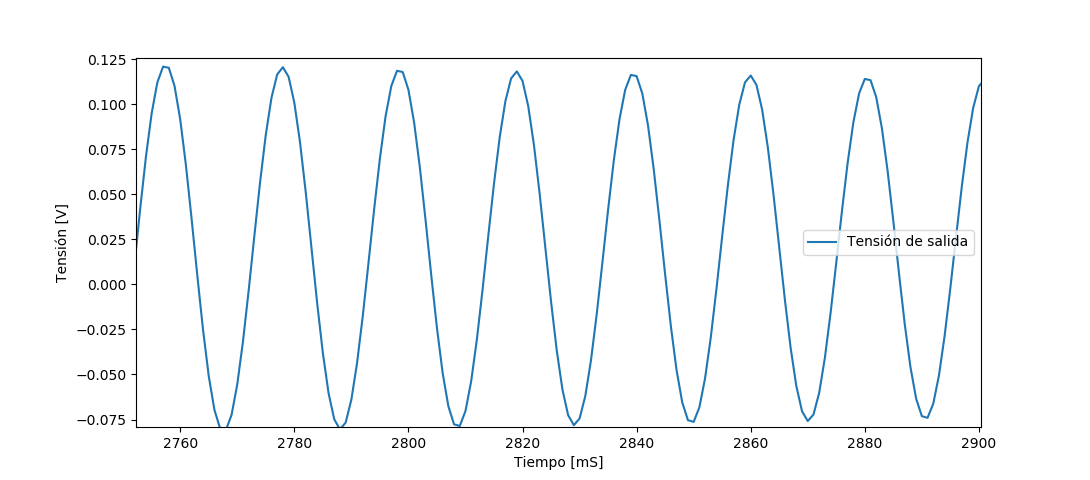
\includegraphics[width=\textwidth]{ImagenesEjercicio4/uniformResponseDETAIL.PNG}
\caption{Respuesta a ruido uniforme detalle, $L=50$.}
	\label{fig:uniformed}
\end{figure}
Finalmente se ingresó al sistema con ruido Binario aleatorio.
\begin{figure}[H]
	\centering
	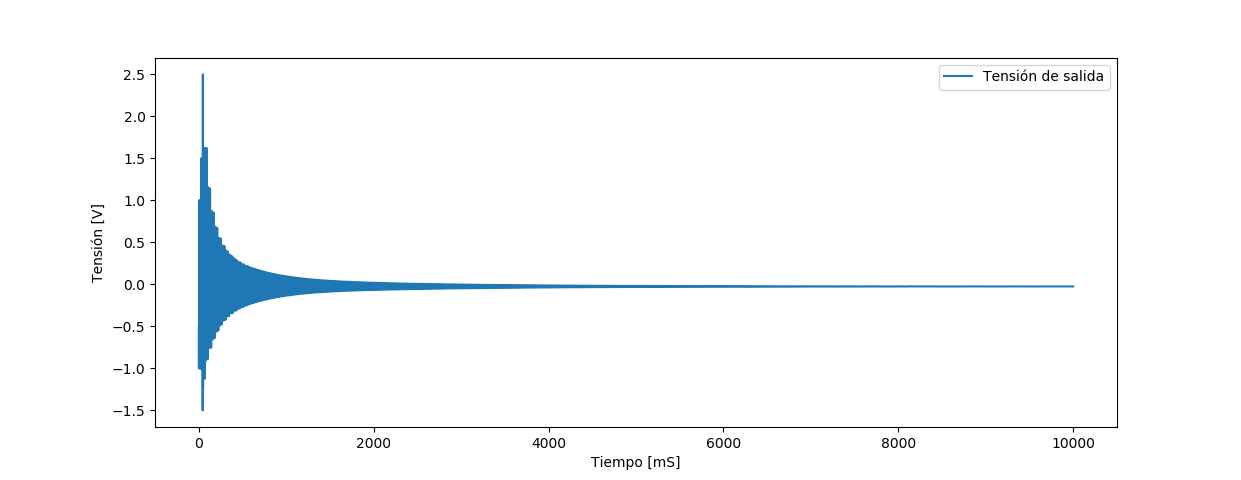
\includegraphics[width=\textwidth]{ImagenesEjercicio4/binaryResponse.PNG}
\caption{Respuesta a ruido Binario, L=50.}
	\label{fig:binary}
\end{figure}

Se puede observar en la Figura (\ref{fig:binary}) que existe una envolvente mucho más severa que las anteriores. Ademas, a mediad que el tiempo aumenta, el valor de tensión tiende cercano a cero, lo cual es un efecto deseado.
\begin{figure}[H]
	\centering
	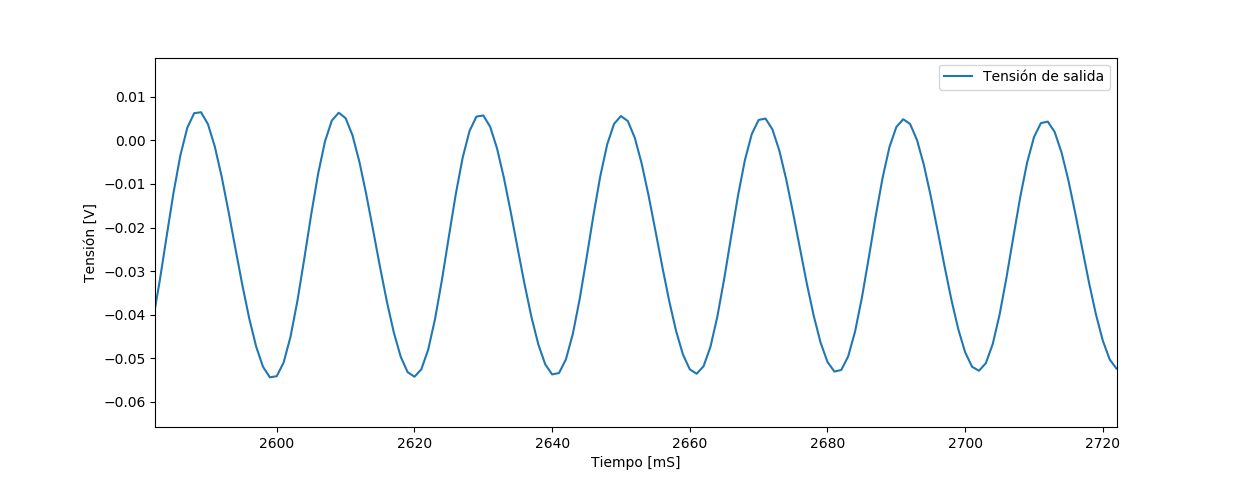
\includegraphics[width=\textwidth]{ImagenesEjercicio4/binaryResponseDETAIL.PNG}
	\caption{Respuesta a ruido Binario en detalle , $L=50$.}
	\label{fig:binaryD}
\end{figure}

Adicionalmente se computó la respuesta impulsiva del sistema, siendo esta:
\begin{figure}[H]
	\centering
	\includegraphics[width=\textwidth]{ImagenesEjercicio4/impulseResponse.PNG}
	\caption{Respuesta al Impulso, $L=50$.}
	\label{fig:impulse}
\end{figure}

Vale la pena mencionar que la salida nunca es negativa, esto se debe a que cuando la excitación es únicamente positiva, dado que la realimentación es positiva y que no existe ninguna inversión de fase, la salida siempre resulta positiva. Así también se muestra un detalle de la respuesta.
\begin{figure}[H]
	\centering
	\includegraphics[width=\textwidth]{ImagenesEjercicio4/impulseResponseDETAIL.PNG}
	\caption{Respuesta al Impulso detalle, $L=50$.}
	\label{fig:impulsed}
\end{figure}

También cabe destacar que la ``velocity'' fue introducida no solo al final de la sintetización como modulador de volumen, sino también en el ruido del comienzo, dado que dicha propiedad, en la guitarra, simboliza la intensidad con la cual fue tocada la cuerda.

\subsubsection{Estabilidad}
La estabilidad del sistema es determinada por la Ecuación (\ref{eq:hzks}). Se puede observar que si $RL$ es mayor o igual a la unidad, el sistema es inestable. Si bien, teóricamente es cierto, en la realidad se encuentra que si se da dicha condición, no solo no se provoca inestabilidad, sino que es preferible este valor dado, ya que logra extender las oscilaciones un mayor tiempo.
%no solo no provocará inestabilidad, sino que es recomendable este valor dado que logrará extender las oscilaciones  un mayor tiempo.
%WUT? TRADUJE BIEN?

\subsection{Mejora propuesta}
El sistema anterior cuenta con algunas limitaciones. Un claro ejemplo de esto es la frecuencia,
a cual para valores pequeños de $L$, la diferencia entre $f_r(L)$ y $f_r(L+1)$ resulta grande, dejando una banda de frecuencias sin poder ser sintonizadas, como ejemplifica la siguiente imagen.
\begin{figure}[H]	
	\centering
	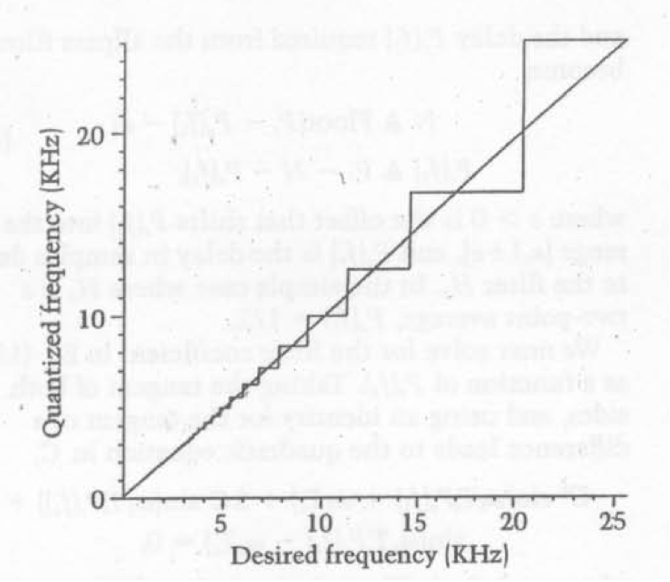
\includegraphics[width=0.6\textwidth]{ImagenesEjercicio4/sintfreq.PNG}
	\caption{Dificultad en sintonización de frecuencia.}
	\label{fig:sintfreq}
\end{figure}

Otro defecto, es el final abrupto con el que cuentan algunas notas. Si se pide una duración reducida,  las discontinuidades en el sonido provocan un efecto indeseado.

\subsubsection{Sintonización de frecuencia}
Para definir la frecuencia de resonancia del sistema, dado que la Ecuación (\ref{eq:fr}) no deja grados de libertad, ya que la frecuencia de muestreo es fija, lo único que se puede hacer es realizar una modificación al circuito. El nuevo modelo propuesto es el siguiente:
\begin{figure}[H]
	\centering
	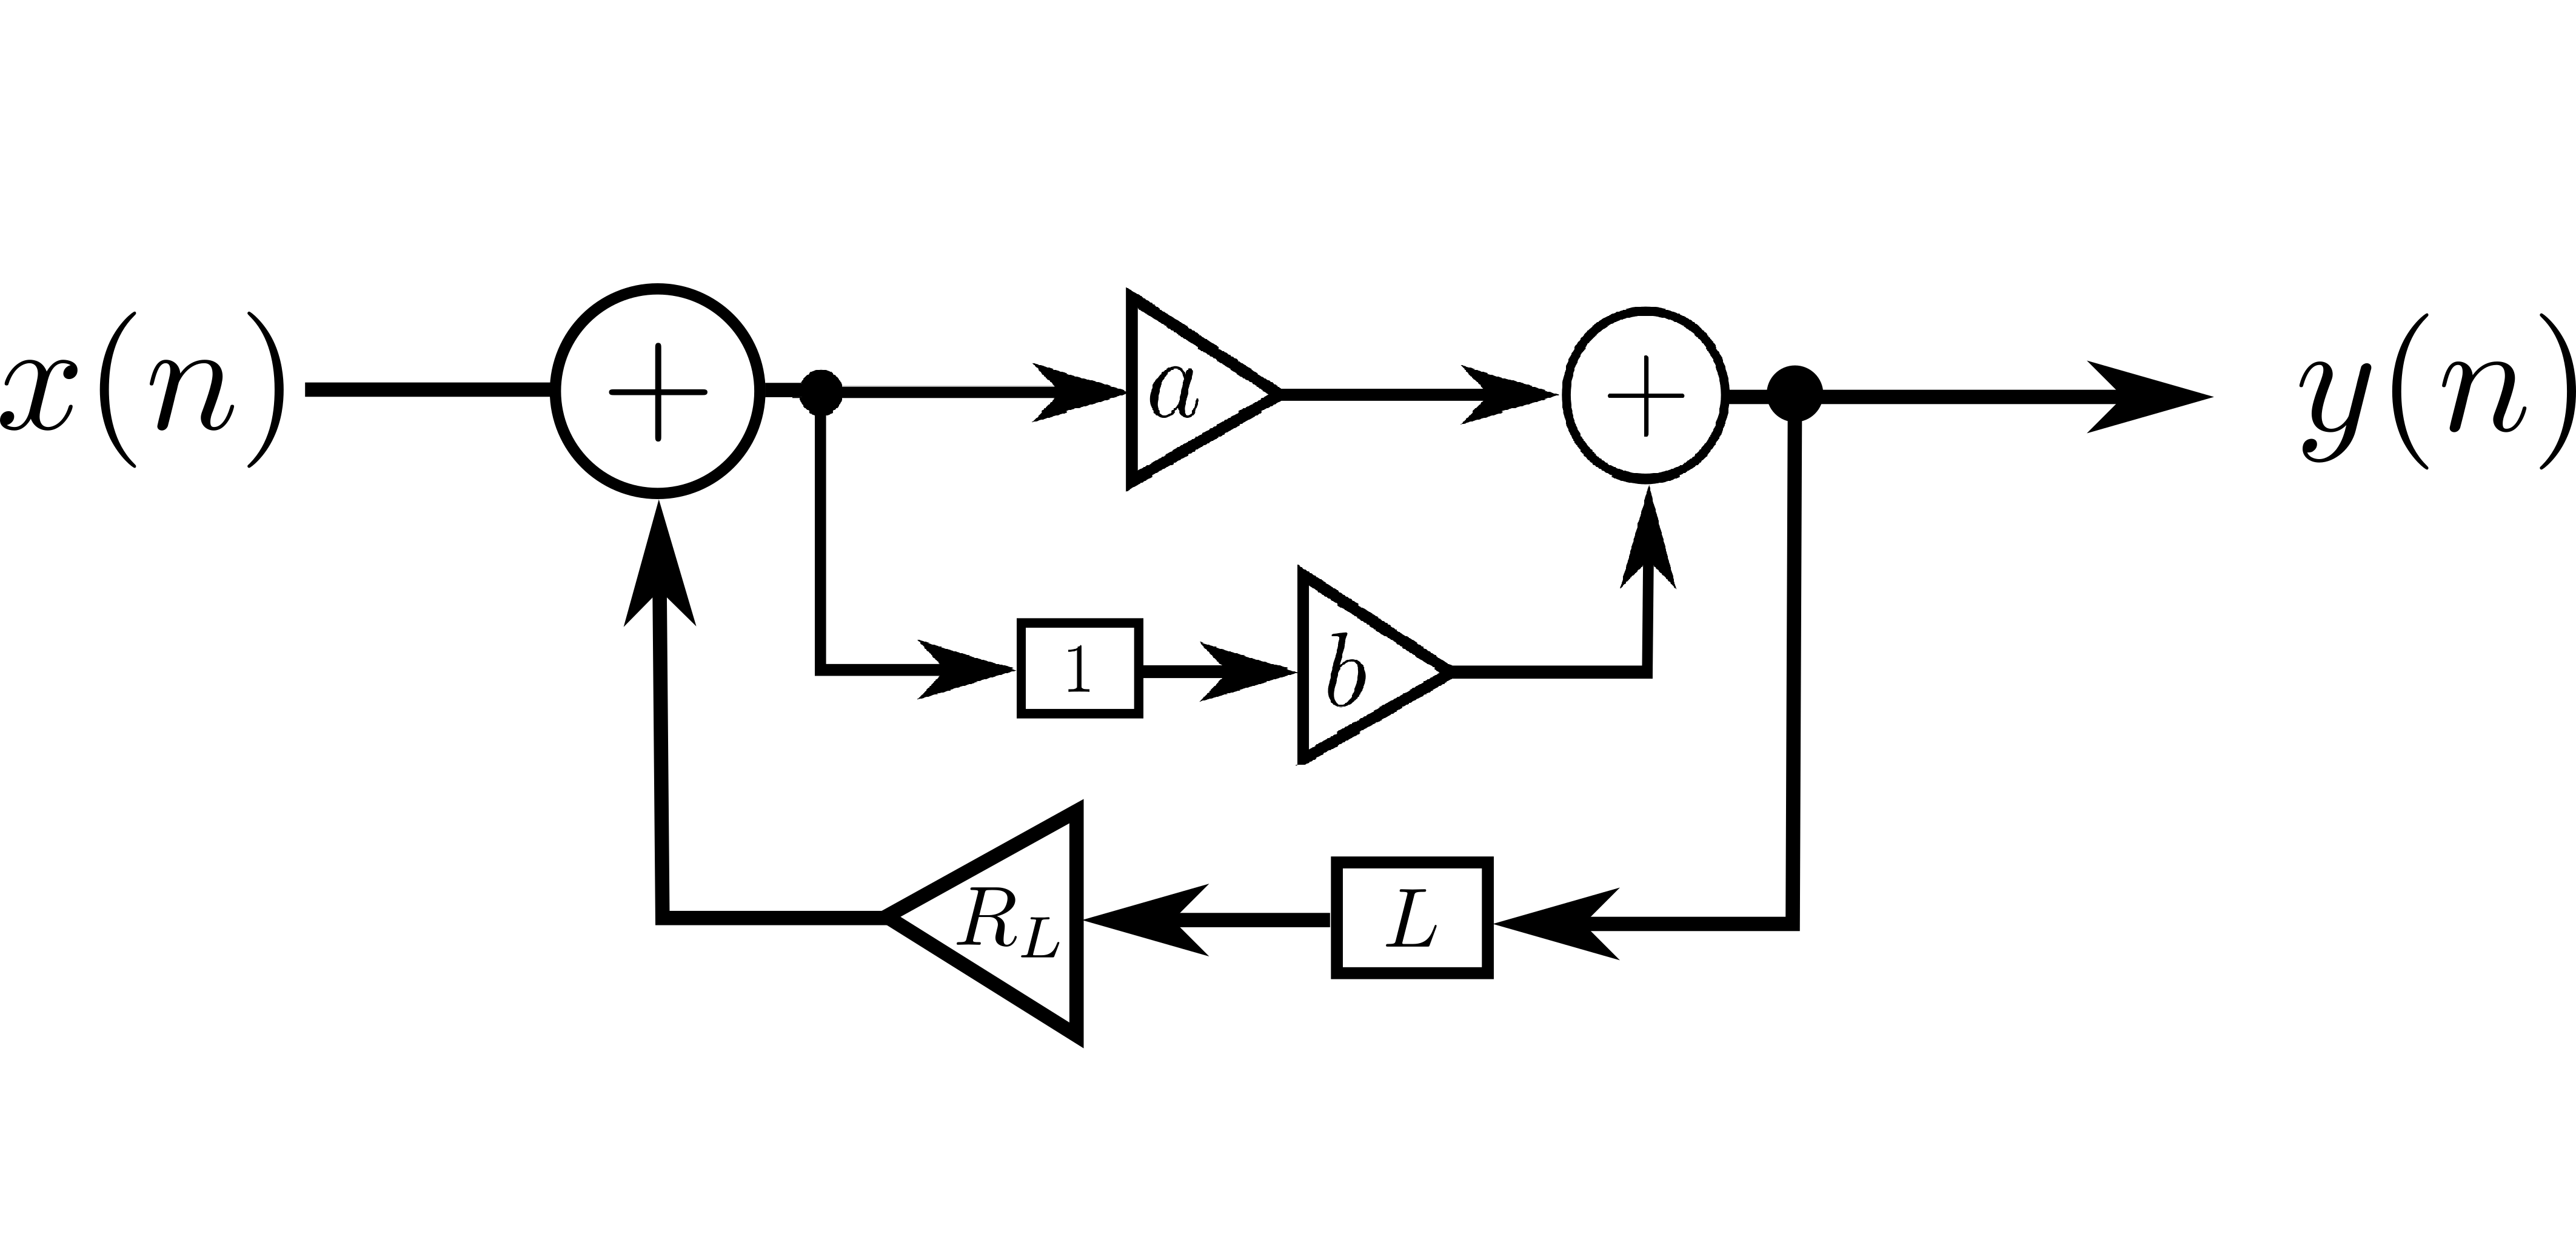
\includegraphics[width=0.8\textwidth]{ImagenesEjercicio4/mejoraks.PNG}
	\caption{Algoritmo Karplus-Strong mejora propuesta.}
	\label{fig:ksmejora}
\end{figure}

Utilizando esta propuesta se puede obtener la ecuación en diferencias del sistema, siendo esta:
\begin{align}
y(n) = a\cdot x(n) +b\cdot x(n-1) + a\cdot R_L \cdot y(n-L)+b\cdot R_L \cdot y(n-L-1) 
\end{align}

Nótese, que si $a=b=$ $\frac{1}{2}$ el sistema coincide con el original. Utilizando el mismo razonamiento, se llega a que la nueva frecuencia de resonancia es:
\begin{align}
f_r=\frac{f_s}{L\cdot (a+b)+b}
\end{align}

Se debe eligir apropiadamente $a$ y $b$, teniendo en cuenta que su suma debe de dar 1 para que el sistema sea el promedio ponderado realizado por estos sea realmente un promedio.

Un punto en contra de esta solución es que, dependiendo de los valores de $a$ y $b$, se toma más en consideración una u otra linea del promedio.

\subsubsection{Continuidad del sonido}
Se tuvo en cuenta que el sonido sea una función suave, dado que cambios bruscos en el sonido no son placenteros ni esperados en la sintetización que es deseada implementar. Para lidiar con este problema lo que se realizo fue definir un factor de ventana, a partir de la cual se atenuá gradualmente el sonido hasta que sea nulo. Para esto se definió una ventana que tiene valor unitario para valores de tiempo menores al factor de ventana especificado, mientras que para valores superiores, decae gradualmente con una función cosenoidal, barriendo desde 0 a $\frac{\pi}{2}$ como se ilustra a continuación.
\begin{figure}[H]
	\centering
	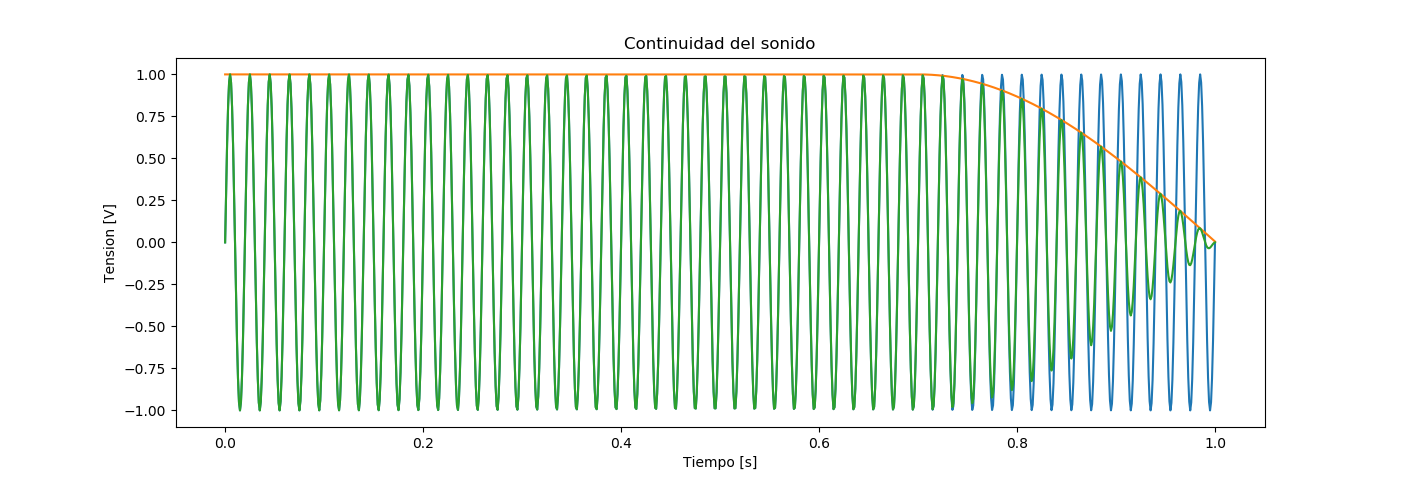
\includegraphics[width=1\textwidth]{ImagenesEjercicio4/continuidad.PNG}
	\caption{Muestra del factor de ventana.}
	\label{fig:windowfactor}
\end{figure}

De esta forma se aumenta la calidad de la síntesis en gran medida si se combina con la idea de que la duración de la nota y la del sonido son cosas distintas.

\subsubsection{Caja de resonancia}
La caja de resonancia es una parte primordial de la gran mayoría de instrumentos acústicos, principalmente de cuerda y percusión. Tiene la finalidad de amplificar o modular un sonido (en los instrumentos de cuerda generalmente a través de un puente). Los instrumentos que cubren rangos de sonidos más graves, como el contrabajo, el violonchelo o el bombo, necesitan una caja de resonancia bastante mayor que el resto.

La necesidad de utilizar una caja de resonancia en una guitarra se debe justamente a que la vibración de las cuerdas, que generan los frente de onda esféricos propios del sonido, tienen una gran dificultad para propagarse por el medio (el aire) debido a su reducida amplitud.

La manera en la cual este elemento sopesa dicho problema es capturando parte del frente de onda en su cavidad. Allí las frecuencias producidas por las cuerdas son amplificadas en igual magnitud y luego liberadas al medio con la intensidad suficiente para que pueda propagarse y que sea apreciable el sonido.

Finalmente cabe destacar que en el ámbito de señales realmente no es necesario dicha caja, al igual que tampoco un filtro que la emule, debido a que su función es amplificar, efecto que se puede hacer digitalmente sin ningún problema. 

\subsection{Karplus-Strong percusión}
Se puede realizar una modificación al modelo inicial agregando un factor aleatorio como se observa a continuación:
\begin{figure}[H]
	\centering
	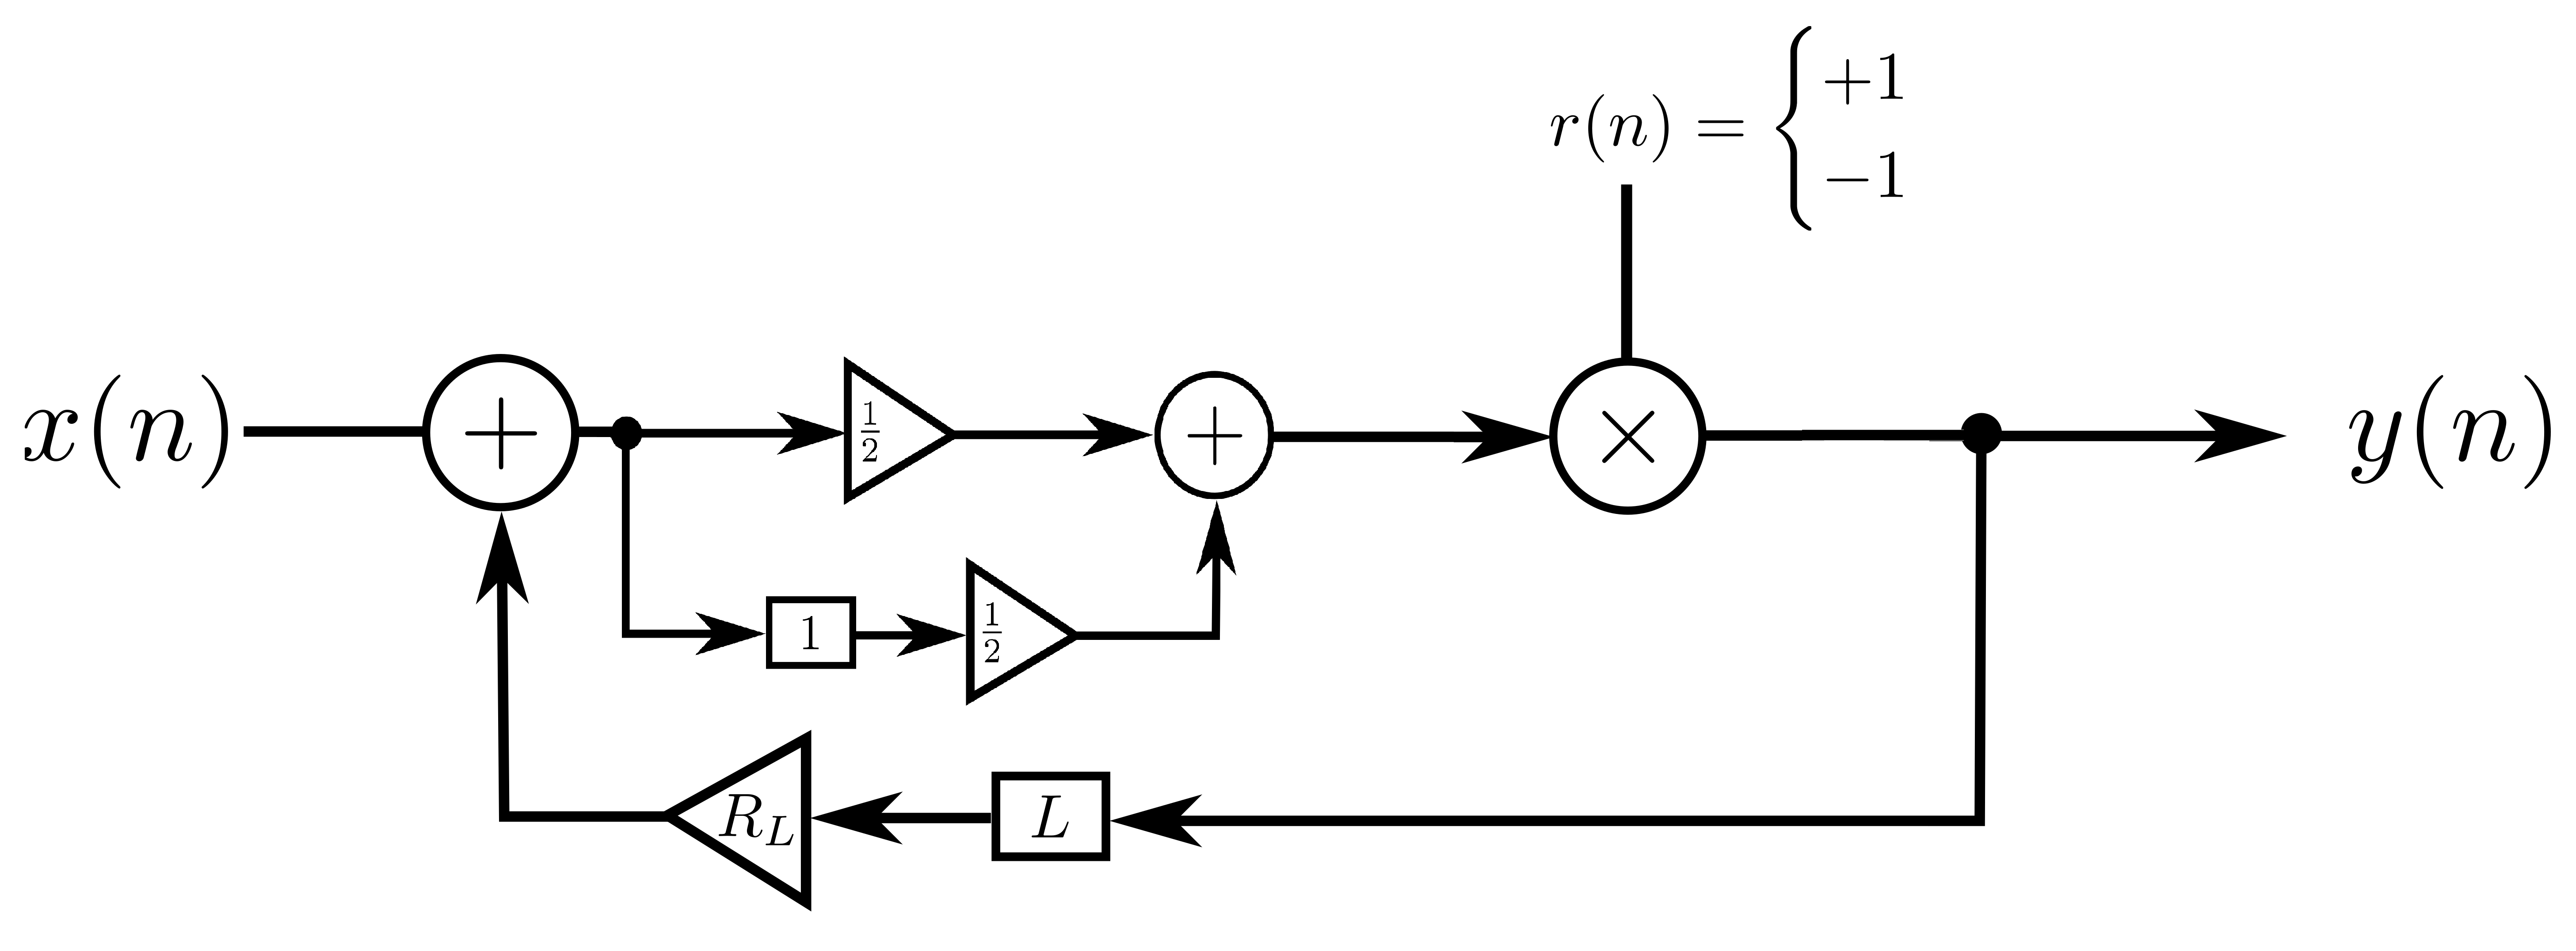
\includegraphics[width=1\textwidth]{ImagenesEjercicio4/ksdrum.PNG}
	\caption{Karplus-Strong percusión.}
	\label{fig:KSPERC}
\end{figure}

El valor de $b$ indica el nivel de cambio para el sonido final. Vale la pena notar que si $b=1$, el algoritmo resulta igual al original. Para obtener sonidos de percusión se utiliza un valor de $b=0,5$.

Una gran diferencia entre la guitarra sintetizada y un elemento de percusión es que estos últimos no cuentan con ``notas'', sino que tienen un sonido característico, para obtener un sonido similar a un elemento de percusión se utilizan valores elevados de $L$.

\subsection{Espectrogramas}
Finalmente se realizaron espectrogramas de tanto la guitarra como el ``redoblante'' obteniendo los siguientes resultados.
\begin{figure}[H]
	\centering
	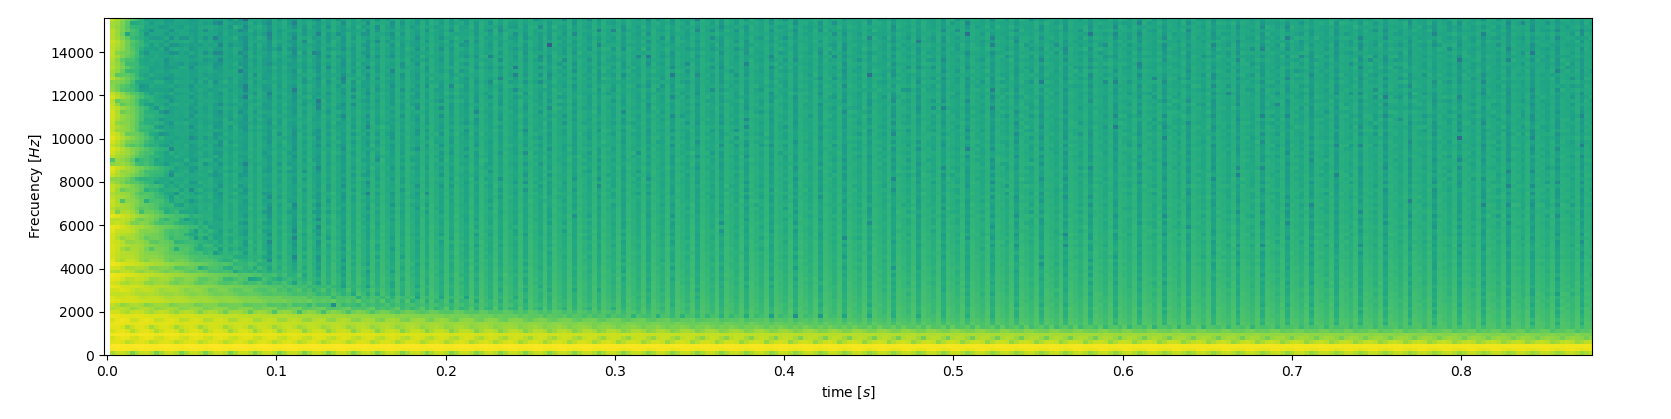
\includegraphics[width=1\textwidth]{ImagenesEjercicio4/espectroGuitar.PNG}
	\caption{Espectrograma Guitarra.}
	\label{fig:especGuitar}
\end{figure}
\begin{figure}[H]
	\centering
	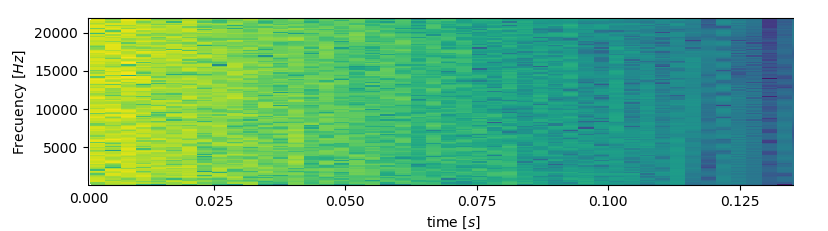
\includegraphics[width=1\textwidth]{ImagenesEjercicio4/espectroDrum.PNG}
	\caption{Espectrograma Redoblante.}
	\label{fig:especdrum}
\end{figure}

Se puede diferenciar que la guitarra cuenta con mayor densidad armónica de baja frecuencia al igual que se extiende considerablemente mas en el tiempo, mientra que el redoblante cuenta con mayor contenido de alta frecuencia y su duración es mucho menor.